\documentclass[12pt, a4paper]{article}

% ─── Packages ─────────────────────────────────────────────
\usepackage[utf8]{inputenc}
\usepackage[T1]{fontenc}
\usepackage[english]{babel}
\usepackage{lmodern}
\usepackage[left=2.5cm, right=2.5cm, top=2.5cm, bottom=2.5cm]{geometry}
\usepackage{setspace}
\usepackage{parskip}
\usepackage{enumitem}
\usepackage{booktabs}
\usepackage{tabularx}
\usepackage{array}
\usepackage{hyperref}
\usepackage{amsmath}
\usepackage{xcolor}
\usepackage{listings}
\usepackage{float}
\usepackage{tikz}
\usepackage{subcaption}

\usetikzlibrary{
    arrows.meta,
    positioning,
    shapes.geometric,
    shapes.multipart,
    fit,
    backgrounds,
    calc,
    decorations.pathreplacing,
    patterns
}

\hypersetup{
    colorlinks=true,
    linkcolor=blue!60!black,
    citecolor=blue!60!black,
    urlcolor=blue!60!black,
}

\onehalfspacing

% ─── Colors ───────────────────────────────────────────────
\definecolor{inputcolor}{HTML}{E3F2FD}
\definecolor{corecolor}{HTML}{FFF3E0}
\definecolor{outputcolor}{HTML}{E8F5E9}
\definecolor{compbg}{HTML}{F5F5F5}
\definecolor{compborder}{HTML}{9E9E9E}
\definecolor{accentblue}{HTML}{1565C0}
\definecolor{accentorange}{HTML}{E65100}
\definecolor{accentgreen}{HTML}{2E7D32}
\definecolor{costred}{HTML}{C62828}
\definecolor{cachegold}{HTML}{F9A825}
\definecolor{yamlbg}{HTML}{FAFAFA}
\definecolor{yamlkey}{HTML}{0D47A1}
\definecolor{yamlstr}{HTML}{1B5E20}
\definecolor{yamlcomment}{HTML}{757575}
\definecolor{jsonbg}{HTML}{F5F5F5}

% ─── Listings ─────────────────────────────────────────────
\lstdefinestyle{yaml}{
    backgroundcolor=\color{yamlbg},
    basicstyle=\ttfamily\scriptsize,
    breaklines=true,
    frame=single,
    rulecolor=\color{compborder},
    commentstyle=\color{yamlcomment}\itshape,
    keywordstyle=\color{yamlkey}\bfseries,
    stringstyle=\color{yamlstr},
    morecomment=[l]{\#},
    columns=fullflexible,
    xleftmargin=4pt,
    xrightmargin=4pt,
    aboveskip=8pt,
    belowskip=8pt,
    tabsize=2,
    showstringspaces=false,
}

\lstdefinestyle{json}{
    backgroundcolor=\color{jsonbg},
    basicstyle=\ttfamily\scriptsize,
    breaklines=true,
    frame=single,
    rulecolor=\color{compborder},
    keywordstyle=\color{yamlkey}\bfseries,
    stringstyle=\color{yamlstr},
    columns=fullflexible,
    xleftmargin=4pt,
    xrightmargin=4pt,
    aboveskip=8pt,
    belowskip=8pt,
    tabsize=2,
    showstringspaces=false,
}

\lstdefinestyle{python}{
    backgroundcolor=\color{yamlbg},
    basicstyle=\ttfamily\scriptsize,
    breaklines=true,
    frame=single,
    rulecolor=\color{compborder},
    keywordstyle=\color{accentblue}\bfseries,
    stringstyle=\color{yamlstr},
    commentstyle=\color{yamlcomment}\itshape,
    columns=fullflexible,
    xleftmargin=4pt,
    xrightmargin=4pt,
    aboveskip=8pt,
    belowskip=8pt,
    tabsize=4,
    showstringspaces=false,
    language=Python,
}

\lstdefinestyle{jinja}{
    backgroundcolor=\color{yamlbg},
    basicstyle=\ttfamily\scriptsize,
    breaklines=true,
    frame=single,
    rulecolor=\color{compborder},
    columns=fullflexible,
    xleftmargin=4pt,
    xrightmargin=4pt,
    aboveskip=8pt,
    belowskip=8pt,
    tabsize=2,
    showstringspaces=false,
    moredelim=[s][\color{accentorange}\bfseries]{\{\{}{\}\}},
    moredelim=[s][\color{accentorange}\bfseries]{\{{\%}}{\%\}},
}

\lstdefinestyle{directory}{
    backgroundcolor=\color{yamlbg},
    basicstyle=\ttfamily\scriptsize,
    breaklines=true,
    frame=single,
    rulecolor=\color{compborder},
    columns=fullflexible,
    xleftmargin=4pt,
    xrightmargin=4pt,
    aboveskip=8pt,
    belowskip=8pt,
    showstringspaces=false,
}

% ─── TikZ Styles ─────────────────────────────────────────
\tikzset{
    component/.style={
        rectangle, draw=compborder, fill=compbg,
        rounded corners=3pt, minimum height=1cm,
        minimum width=2.8cm, align=center,
        font=\small\sffamily
    },
    component wide/.style={
        component, minimum width=4cm
    },
    layer box/.style={
        rectangle, draw=#1!60!black, fill=#1!8,
        rounded corners=5pt, inner sep=10pt,
        line width=1pt
    },
    layer label/.style={
        font=\small\sffamily\bfseries, text=#1!60!black
    },
    data flow/.style={
        -{Stealth[length=6pt]}, thick, color=#1!60!black
    },
    data flow/.default={black},
    bidirectional/.style={
        {Stealth[length=5pt]}-{Stealth[length=5pt]}, thick, color=#1!60!black
    },
    bidirectional/.default={black},
    input file/.style={
        rectangle, draw=accentblue!70, fill=inputcolor,
        rounded corners=2pt, minimum height=0.9cm,
        minimum width=2.4cm, align=center,
        font=\small\sffamily
    },
    output file/.style={
        rectangle, draw=accentgreen!70, fill=outputcolor,
        rounded corners=2pt, minimum height=0.9cm,
        minimum width=2.4cm, align=center,
        font=\small\sffamily
    },
    process/.style={
        rectangle, draw=accentorange!70, fill=corecolor,
        rounded corners=2pt, minimum height=0.9cm,
        minimum width=2.4cm, align=center,
        font=\small\sffamily
    },
    provider/.style={
        rectangle, draw=compborder, fill=white,
        rounded corners=2pt, minimum height=0.7cm,
        minimum width=1.6cm, align=center,
        font=\scriptsize\sffamily
    },
    orchstep/.style={
        rectangle, draw=accentblue!50, fill=accentblue!5,
        rounded corners=2pt, minimum height=0.6cm,
        align=left, font=\scriptsize\sffamily,
        text width=6cm
    },
}

% ─── Title ────────────────────────────────────────────────
\title{%
    \vspace{-1cm}
    \textbf{Architecture Draft}\\[0.6em]
    \Large Cost-Efficient LLM-Based\\
    Multi-Agent Simulation Framework\\[0.8em]
    \normalsize\textit{Working Document --- Master's Thesis}
}
\author{Janik H\"ausser}
\date{May 2026}

% ──────────────────────────────────────────────────────────
\begin{document}

\maketitle
\thispagestyle{empty}
\vfill
\begin{center}
    \textit{Draft for discussion --- subject to change during implementation.}
\end{center}
\newpage

\setcounter{page}{1}
\tableofcontents
\newpage

% ══════════════════════════════════════════════════════════
\section{System Overview}
\label{sec:overview}
% ══════════════════════════════════════════════════════════

The framework follows a three-layer architecture: an \textbf{input layer} for declarative scenario and persona definitions, a \textbf{core engine} for orchestration, LLM interaction, and cost control, and an \textbf{output layer} for structured, reproducible results.

\begin{figure}[H]
\centering
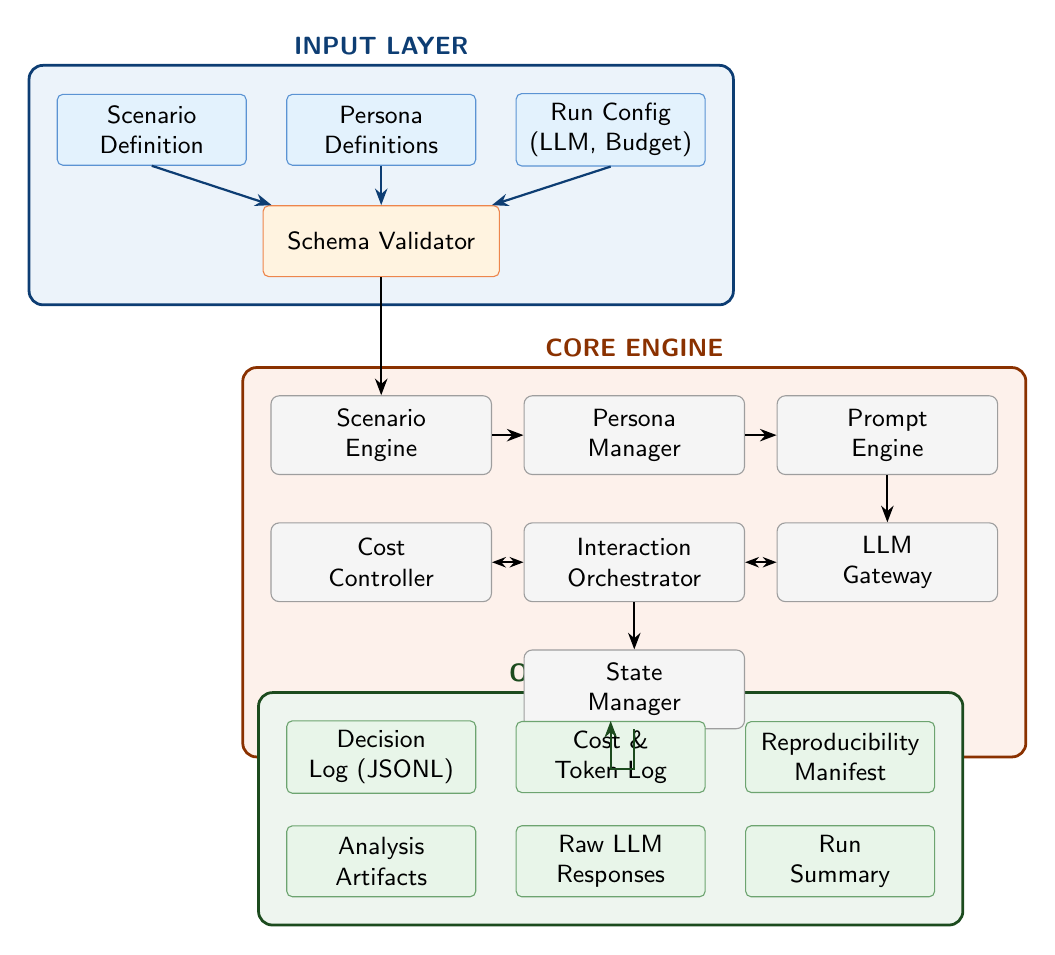
\begin{tikzpicture}[node distance=0.6cm and 0.8cm]

    % ── Input Layer ──
    \node[input file] (scenario) {Scenario\\Definition};
    \node[input file, right=0.5cm of scenario] (personas) {Persona\\Definitions};
    \node[input file, right=0.5cm of personas] (runconfig) {Run Config\\(LLM, Budget)};

    \node[process, below=0.5cm of personas, minimum width=3cm] (validator) {Schema Validator};

    \begin{scope}[on background layer]
        \node[layer box=accentblue, fit=(scenario)(personas)(runconfig)(validator),
              label={[layer label=accentblue]above:INPUT LAYER}] (inputlayer) {};
    \end{scope}

    \draw[data flow=accentblue] (scenario.south) -- (validator);
    \draw[data flow=accentblue] (personas.south) -- (validator);
    \draw[data flow=accentblue] (runconfig.south) -- (validator);

    % ── Core Engine ──
    \node[component, below=1.5cm of validator] (sceneng) {Scenario\\Engine};
    \node[component, right=0.4cm of sceneng] (persmgr) {Persona\\Manager};
    \node[component, right=0.4cm of persmgr] (prompteng) {Prompt\\Engine};

    \node[component, below=0.6cm of sceneng] (costctrl) {Cost\\Controller};
    \node[component, right=0.4cm of costctrl] (orchestrator) {Interaction\\Orchestrator};
    \node[component, right=0.4cm of orchestrator] (llmgw) {LLM\\Gateway};

    \node[component, below=0.6cm of orchestrator] (statemgr) {State\\Manager};

    \begin{scope}[on background layer]
        \node[layer box=accentorange,
              fit=(sceneng)(persmgr)(prompteng)(costctrl)(orchestrator)(llmgw)(statemgr),
              label={[layer label=accentorange]above:CORE ENGINE}] (corelayer) {};
    \end{scope}

    \draw[data flow] (validator) -- (sceneng);
    \draw[data flow] (sceneng) -- (persmgr);
    \draw[data flow] (persmgr) -- (prompteng);
    \draw[data flow] (prompteng) -- (llmgw);
    \draw[bidirectional] (costctrl) -- (orchestrator);
    \draw[bidirectional] (orchestrator) -- (llmgw);
    \draw[data flow] (orchestrator) -- (statemgr);

    % ── Output Layer ──
    \node[output file, below=1.5cm of costctrl] (declog) {Decision\\Log (JSONL)};
    \node[output file, right=0.5cm of declog] (costlog) {Cost \&\\Token Log};
    \node[output file, right=0.5cm of costlog] (manifest) {Reproducibility\\Manifest};

    \node[output file, below=0.4cm of declog] (analysis) {Analysis\\Artifacts};
    \node[output file, right=0.5cm of analysis] (rawresp) {Raw LLM\\Responses};
    \node[output file, right=0.5cm of rawresp] (summary) {Run\\Summary};

    \begin{scope}[on background layer]
        \node[layer box=accentgreen,
              fit=(declog)(costlog)(manifest)(analysis)(rawresp)(summary),
              label={[layer label=accentgreen]above:OUTPUT LAYER}] (outputlayer) {};
    \end{scope}

    \draw[data flow=accentgreen] (statemgr.south) -- ++(0,-0.5) -| (costlog.north);

\end{tikzpicture}
\caption{High-level three-layer architecture of the simulation framework.}
\label{fig:overview}
\end{figure}

% ══════════════════════════════════════════════════════════
\section{Input Layer: Schema Definitions}
\label{sec:input}
% ══════════════════════════════════════════════════════════

The framework accepts \textbf{three YAML configuration files} as input, each validated against a JSON Schema before processing. This ensures configuration errors are caught immediately---before any costly API calls are made.

\begin{figure}[H]
\centering
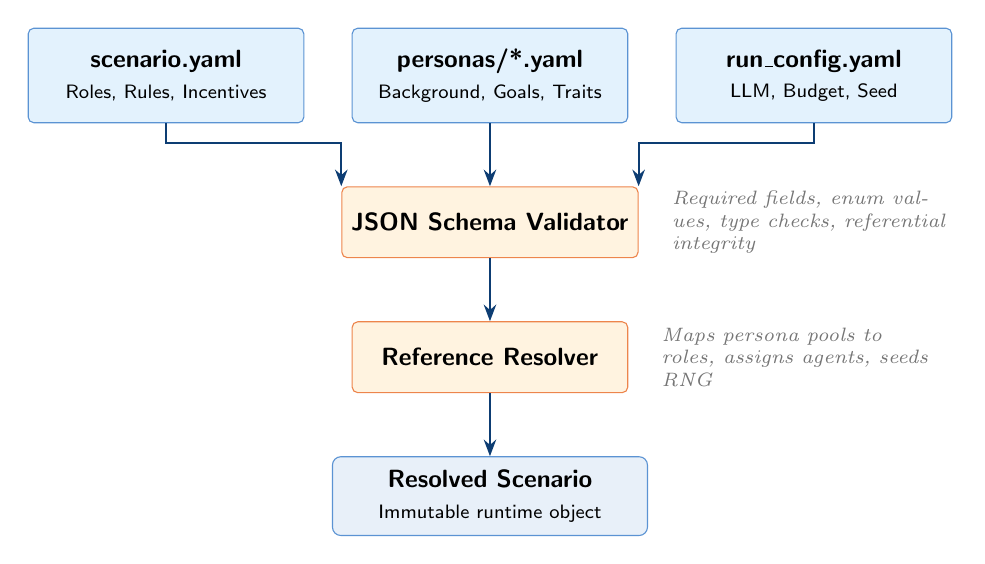
\begin{tikzpicture}[node distance=0.4cm and 0.6cm]
    \node[input file, minimum width=3.5cm, minimum height=1.2cm] (sc) {
        \textbf{scenario.yaml}\\
        {\scriptsize Roles, Rules, Incentives}
    };
    \node[input file, minimum width=3.5cm, minimum height=1.2cm, right=0.6cm of sc] (pe) {
        \textbf{personas/*.yaml}\\
        {\scriptsize Background, Goals, Traits}
    };
    \node[input file, minimum width=3.5cm, minimum height=1.2cm, right=0.6cm of pe] (rc) {
        \textbf{run\_config.yaml}\\
        {\scriptsize LLM, Budget, Seed}
    };

    \node[process, below=0.8cm of pe, minimum width=3.5cm] (val) {\textbf{JSON Schema Validator}};

    \node[process, below=0.8cm of val, minimum width=3.5cm] (resolve) {\textbf{Reference Resolver}};

    \node[component wide, below=0.8cm of resolve, draw=accentblue!70, fill=accentblue!10] (resolved) {
        \textbf{Resolved Scenario}\\
        {\scriptsize Immutable runtime object}
    };

    \draw[data flow=accentblue] (sc.south) -- ++(0,-0.25) -| (val.north west);
    \draw[data flow=accentblue] (pe.south) -- (val.north);
    \draw[data flow=accentblue] (rc.south) -- ++(0,-0.25) -| (val.north east);
    \draw[data flow=accentblue] (val) -- (resolve);
    \draw[data flow=accentblue] (resolve) -- (resolved);

    % Annotations
    \node[right=0.3cm of val, font=\scriptsize\itshape, text=yamlcomment, text width=3.5cm] {
        Required fields, enum values, type checks, referential integrity
    };
    \node[right=0.3cm of resolve, font=\scriptsize\itshape, text=yamlcomment, text width=3.5cm] {
        Maps persona pools to roles, assigns agents, seeds RNG
    };
\end{tikzpicture}
\caption{Input validation and resolution pipeline.}
\label{fig:input-pipeline}
\end{figure}

% ── 2.1 Scenario Definition ──
\subsection{Scenario Definition (\texttt{scenario.yaml})}

Describes the research question, stakeholder roles, interaction rules, and incentive mechanisms in a \textbf{domain-agnostic} format.

\begin{lstlisting}[style=yaml, caption={Scenario definition example: peatland rewetting negotiation.}, label={lst:scenario}]
# scenario.yaml
scenario:
  id: "peatland-rewetting-negotiation"
  version: "1.0"
  name: "Peatland Rewetting Negotiation"
  description: >
    Simulation of negotiations between farmers and public authorities
    regarding the rewetting of drained peatlands. Goal: identify effective
    incentive mechanisms for different farmer types.

  # Shared context visible to all agents
  shared_context: >
    Approx. 92% of peatlands in Germany are drained for agriculture.
    Drained peatlands emit ca. 53 Mt CO2-eq annually. The federal
    government aims to rewet at least 50,000 ha by 2030.

  # Stakeholder roles (references to persona files)
  roles:
    - id: "farmer"
      label: "Farmer / Landowner"
      description: "Owns drained peatland and farms it."
      count: 4
      persona_pool: "personas/farmers.yaml"
    - id: "public_authority"
      label: "Public Authority"
      description: "Offers compensation and regulatory frameworks."
      count: 1
      persona_pool: "personas/authorities.yaml"
    - id: "ngo"
      label: "Environmental NGO"
      description: "Advocates for climate protection."
      count: 1
      persona_pool: "personas/ngos.yaml"

  # Interaction rules
  interaction:
    type: "multi_round_negotiation"   # single_shot | multi_round_negotiation | auction | debate
    topology: "all_to_all"            # all_to_all | pairwise | hub_spoke | custom
    rounds:
      min: 3
      max: 10
      termination_condition: "consensus_or_max_rounds"
    turn_order: "simultaneous"        # sequential | simultaneous | random
    visibility:
      decisions: true
      reasoning: false
      history_depth: "full"           # none | last_round | full

  # Incentive mechanisms (scenario-specific)
  incentives:
    - id: "compensation"
      type: "continuous"
      range: [0, 2000]
      unit: "EUR_per_ha_per_year"
      offered_by: "public_authority"
      target: "farmer"
    - id: "contract_duration"
      type: "discrete"
      options: [5, 10, 15, 20, 30]
      unit: "years"
      offered_by: "public_authority"
      target: "farmer"
    - id: "paludiculture_support"
      type: "binary"
      offered_by: "ngo"
      target: "farmer"
    - id: "regulatory_pressure"
      type: "discrete"
      options: ["none", "voluntary_reporting", "mandatory_timeline", "ban_drainage"]
      offered_by: "public_authority"
      target: "farmer"

  # Target metrics
  objectives:
    - id: "acceptance_rate"
      description: "Fraction of farmers accepting rewetting"
      aggregation: "ratio"
    - id: "min_compensation"
      description: "Minimum compensation at which acceptance occurs"
      aggregation: "per_agent"
    - id: "negotiation_rounds"
      description: "Rounds until agreement (or failure)"
      aggregation: "mean"

  # Global constraints
  constraints:
    - "The public authority has a total budget of 500,000 EUR/year."
    - "Farmers can only accept or reject fully (no partial areas)."
    - "Each agent decides independently."
\end{lstlisting}

% ── 2.2 Persona Definition ──
\subsection{Persona Definitions (\texttt{personas/*.yaml})}

Describes individual agent personalities within a role. Separated from the scenario to enable reuse and combinatorial studies across experiments.

\begin{lstlisting}[style=yaml, caption={Persona definitions for farmer agents (excerpt).}, label={lst:personas}]
# personas/farmers.yaml
personas:
  - id: "conventional_large"
    label: "Conventional Large Farm"
    role: "farmer"
    background: >
      Operates a 200ha arable farm, 60ha on drained peatland.
      Primary income from corn and grain. Heavy investment in
      drainage infrastructure. Two employees, uncertain succession.
    goals:
      primary: "Ensure economic stability of the farm"
      secondary: "Preserve the farm for the next generation"
    risk_profile: "risk_averse"
    decision_factors:
      - factor: "compensation_level"
        weight: "high"
        threshold: "At least 1200 EUR/ha/year to compensate crop loss"
      - factor: "contract_duration"
        weight: "medium"
        preference: "Shorter preferred (max 10 years)"
      - factor: "regulatory_risk"
        weight: "medium"
        sensitivity: "Responds strongly to regulatory pressure"
    personality_traits:
      stubbornness: 0.7
      reciprocity: 0.3
      environmental_concern: 0.2
    constraints:
      - "Can rewet at most 40ha (remaining 20ha adjoin buildings)"

  - id: "ecological_pioneer"
    label: "Ecological Pioneer Farm"
    role: "farmer"
    background: >
      Organic farm with 80ha, partially extensive management.
      Active in regional conservation projects. Views rewetting
      positively but requires financial security.
    goals:
      primary: "Take a leading role in climate protection"
      secondary: "Develop a viable business model for peatland conservation"
    risk_profile: "risk_seeking"
    decision_factors:
      - factor: "compensation_level"
        weight: "medium"
        threshold: "Feasible from 400 EUR/ha/year"
      - factor: "paludiculture_support"
        weight: "high"
        preference: "Wants to launch paludiculture pilot project"
    personality_traits:
      stubbornness: 0.2
      reciprocity: 0.8
      environmental_concern: 0.9
    constraints: []

  - id: "skeptical_traditional"
    label: "Skeptical Traditional Farm"
    role: "farmer"
    background: >
      Third-generation family farm, 120ha arable on peatland.
      Deep distrust of government programs. Experiences with
      broken political promises. "This has been our land since 1950."
    goals:
      primary: "Continue operating the farm unchanged"
      secondary: "Preserve property rights and autonomy"
    risk_profile: "risk_averse"
    decision_factors:
      - factor: "compensation_level"
        weight: "high"
        threshold: "Would need to exceed 1800 EUR/ha/year"
      - factor: "regulatory_pressure"
        weight: "high"
        sensitivity: "Resists coercion but accepts when no alternative"
      - factor: "trust"
        weight: "high"
        note: "Only trusts long-term, binding commitments"
    personality_traits:
      stubbornness: 0.9
      reciprocity: 0.2
      environmental_concern: 0.1
    constraints:
      - "Accepts only if property remains untouched"
      - "No commitment without exit clause"
\end{lstlisting}

% ── 2.3 Run Configuration ──
\subsection{Run Configuration (\texttt{run\_config.yaml})}

Controls technical aspects: LLM provider selection, cost budgets, parallelism, and reproducibility settings.

\begin{lstlisting}[style=yaml, caption={Run configuration with model routing and cost controls.}, label={lst:runconfig}]
# run_config.yaml
run:
  id: "peatland-exp-001"
  seed: 42
  repetitions: 10
  description: "Baseline run: all incentives active"

llm:
  default_provider: "openai"
  default_model: "gpt-4o-mini"
  temperature: 0.7
  max_tokens_per_response: 1024
  response_format: "json"

  # Model routing: cheaper models for simpler tasks
  routing:
    enabled: true
    rules:
      - task: "decision"
        model: "gpt-4o"
        provider: "openai"
      - task: "reasoning_summary"
        model: "gpt-4o-mini"
        provider: "openai"
      - task: "sentiment_check"
        model: "mistral-small-latest"
        provider: "mistral"

  providers:
    openai:
      api_key_env: "OPENAI_API_KEY"
      rate_limit_rpm: 500
    mistral:
      api_key_env: "MISTRAL_API_KEY"
      rate_limit_rpm: 120
    anthropic:
      api_key_env: "ANTHROPIC_API_KEY"
      rate_limit_rpm: 300
    ollama:
      base_url: "http://localhost:11434"

  retry:
    max_retries: 3
    backoff_base_seconds: 1.0
    backoff_max_seconds: 16.0
    retryable_errors: ["rate_limit", "timeout", "server_error"]

cost:
  budget_total_usd: 5.00
  budget_per_repetition_usd: 0.50
  alert_threshold_pct: 80
  abort_on_exceed: true
  track_granularity: "per_call"

caching:
  enabled: true
  strategy: "content_hash"
  backend: "sqlite"
  cache_path: ".cache/llm_responses.db"
  ttl_hours: 168

parallelism:
  max_workers: 4

output:
  base_dir: "output/runs"
  include_raw_responses: true
  include_prompt_snapshots: true
  log_level: "INFO"
\end{lstlisting}

% ── 2.4 Validation ──
\subsection{JSON Schema Validation}

Each YAML file is validated on load against a corresponding JSON Schema:

\begin{table}[H]
\centering
\begin{tabularx}{\textwidth}{lX}
    \toprule
    \textbf{Validation Aspect} & \textbf{Details} \\
    \midrule
    Required fields & \texttt{scenario.id}, \texttt{roles[].id}, \texttt{personas[].background}, etc. \\
    Enum correctness & \texttt{interaction.type} $\in$ \{\texttt{single\_shot}, \texttt{multi\_round\_negotiation}, \ldots\} \\
    Referential integrity & \texttt{roles[].persona\_pool} points to an existing file \\
    Type checks & Numeric ranges, string formats, array lengths \\
    Semantic constraints & $\sum$ \texttt{roles[].count} $\geq 2$ (at least two agents) \\
    \bottomrule
\end{tabularx}
\caption{Validation aspects enforced by JSON Schema.}
\label{tab:validation}
\end{table}

% ══════════════════════════════════════════════════════════
\section{Core Architecture}
\label{sec:core}
% ══════════════════════════════════════════════════════════

\subsection{Project Structure}

\begin{lstlisting}[style=directory, caption={Proposed project directory structure.}]
framework/
  cli.py                        # CLI entry point (typer)
  core/
    scenario_engine.py          # Parse & validate scenario + personas
    persona_manager.py          # Instantiate agents from persona defs
    orchestrator.py             # Interaction round control
    state.py                    # Immutable round state
    types.py                    # Pydantic models for all data structures
  llm/
    gateway.py                  # Unified LLM interface
    providers/
      base.py                  # Abstract provider protocol
      openai.py                # OpenAI implementation
      anthropic.py             # Anthropic implementation
      mistral.py               # Mistral implementation
      ollama.py                # Local models
    router.py                  # Model routing logic
    cache.py                   # Response cache (SQLite)
    cost_tracker.py            # Token & cost tracking
  prompts/
    engine.py                  # Prompt rendering (Jinja2)
    templates/                 # Base templates (system.j2, user.j2, ...)
    compression.py             # History summarization
  output/
    writer.py                  # Structured output generation
    schemas.py                 # Output schemas (Pydantic)
    hasher.py                  # Reproducibility hashing
    analysis.py                # Aggregation & basic visualization
  utils/
    config.py                  # Config loading & merging
    validation.py              # JSON Schema validation
    logging.py                 # Structured logging (structlog)
\end{lstlisting}

% ── 3.2 Interaction Orchestrator ──
\subsection{Interaction Orchestrator}

The orchestrator is the core loop of the simulation. Each round follows seven sequential steps.

\begin{figure}[H]
\centering
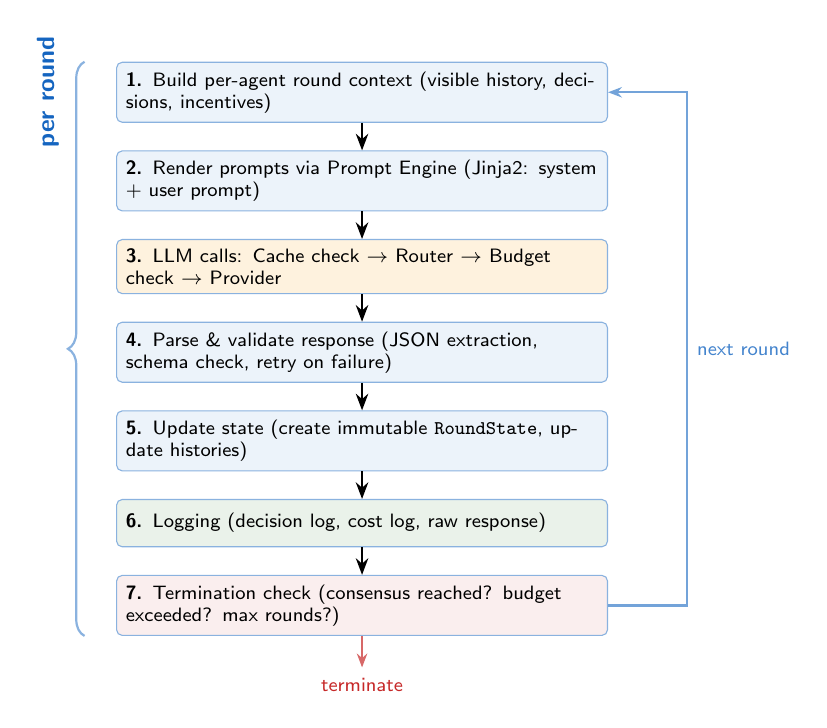
\begin{tikzpicture}[node distance=0.35cm]
    \node[orchstep, fill=accentblue!8] (s1) {\textbf{1.} Build per-agent round context (visible history, decisions, incentives)};
    \node[orchstep, fill=accentblue!8, below=of s1] (s2) {\textbf{2.} Render prompts via Prompt Engine (Jinja2: system + user prompt)};
    \node[orchstep, fill=cachegold!15, below=of s2] (s3) {\textbf{3.} LLM calls: Cache check $\to$ Router $\to$ Budget check $\to$ Provider};
    \node[orchstep, fill=accentblue!8, below=of s3] (s4) {\textbf{4.} Parse \& validate response (JSON extraction, schema check, retry on failure)};
    \node[orchstep, fill=accentblue!8, below=of s4] (s5) {\textbf{5.} Update state (create immutable \texttt{RoundState}, update histories)};
    \node[orchstep, fill=accentgreen!10, below=of s5] (s6) {\textbf{6.} Logging (decision log, cost log, raw response)};
    \node[orchstep, fill=costred!8, below=of s6] (s7) {\textbf{7.} Termination check (consensus reached? budget exceeded? max rounds?)};

    \draw[data flow] (s1) -- (s2);
    \draw[data flow] (s2) -- (s3);
    \draw[data flow] (s3) -- (s4);
    \draw[data flow] (s4) -- (s5);
    \draw[data flow] (s5) -- (s6);
    \draw[data flow] (s6) -- (s7);

    % Loop-back arrow
    \draw[-{Stealth[length=5pt]}, thick, color=accentblue!60]
        (s7.east) -- ++(1,0) |- node[right, pos=0.25, font=\scriptsize\sffamily, text=accentblue!80] {next round} (s1.east);

    % Break arrow
    \draw[-{Stealth[length=5pt]}, thick, color=costred!70]
        (s7.south) -- ++(0,-0.4) node[below, font=\scriptsize\sffamily, text=costred] {terminate};

    % Round label
    \node[left=0.6cm of s1, font=\small\sffamily\bfseries, text=accentblue, rotate=90, anchor=south] {per round};

    % Brace
    \draw[decorate, decoration={brace, amplitude=6pt, mirror}, thick, accentblue!50]
        ([xshift=-0.4cm]s1.north west) -- ([xshift=-0.4cm]s7.south west);
\end{tikzpicture}
\caption{Seven-step orchestrator loop executed per simulation round.}
\label{fig:orchestrator}
\end{figure}

% ── Interaction Topologies ──
\subsection{Interaction Topologies}

The framework supports configurable communication topologies that determine which agents can observe each other's decisions.

\begin{figure}[H]
\centering
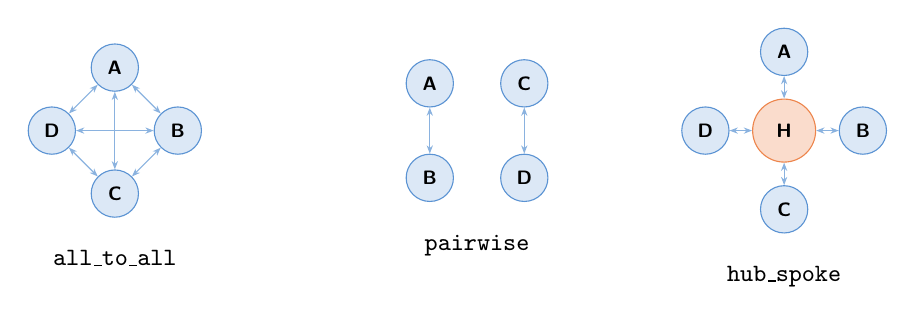
\begin{tikzpicture}[
    agent/.style={circle, draw=accentblue!70, fill=accentblue!15, minimum size=0.6cm, font=\scriptsize\sffamily\bfseries},
    hub/.style={circle, draw=accentorange!70, fill=accentorange!20, minimum size=0.8cm, font=\scriptsize\sffamily\bfseries},
    conn/.style={{Stealth[length=3pt]}-{Stealth[length=3pt]}, thin, accentblue!50},
]
    % All-to-all
    \begin{scope}[local bounding box=ata]
        \node[agent] (a1) at (0, 0.8) {A};
        \node[agent] (a2) at (0.8, 0) {B};
        \node[agent] (a3) at (0, -0.8) {C};
        \node[agent] (a4) at (-0.8, 0) {D};
        \draw[conn] (a1) -- (a2);
        \draw[conn] (a2) -- (a3);
        \draw[conn] (a3) -- (a4);
        \draw[conn] (a4) -- (a1);
        \draw[conn] (a1) -- (a3);
        \draw[conn] (a2) -- (a4);
    \end{scope}
    \node[below=0.3cm of ata, font=\small\sffamily] {\texttt{all\_to\_all}};

    % Pairwise
    \begin{scope}[local bounding box=pw, xshift=4cm]
        \node[agent] (b1) at (0, 0.6) {A};
        \node[agent] (b2) at (0, -0.6) {B};
        \node[agent] (b3) at (1.2, 0.6) {C};
        \node[agent] (b4) at (1.2, -0.6) {D};
        \draw[conn] (b1) -- (b2);
        \draw[conn] (b3) -- (b4);
    \end{scope}
    \node[below=0.3cm of pw, font=\small\sffamily] {\texttt{pairwise}};

    % Hub-spoke
    \begin{scope}[local bounding box=hs, xshift=8.5cm]
        \node[hub] (h) at (0, 0) {H};
        \node[agent] (c1) at (0, 1) {A};
        \node[agent] (c2) at (1, 0) {B};
        \node[agent] (c3) at (0, -1) {C};
        \node[agent] (c4) at (-1, 0) {D};
        \draw[conn] (h) -- (c1);
        \draw[conn] (h) -- (c2);
        \draw[conn] (h) -- (c3);
        \draw[conn] (h) -- (c4);
    \end{scope}
    \node[below=0.3cm of hs, font=\small\sffamily] {\texttt{hub\_spoke}};

\end{tikzpicture}
\caption{Supported interaction topologies. \texttt{custom} (not shown) uses an adjacency matrix.}
\label{fig:topologies}
\end{figure}

\begin{table}[H]
\centering
\begin{tabularx}{\textwidth}{llX}
    \toprule
    \textbf{Topology} & \textbf{Description} & \textbf{Use Case} \\
    \midrule
    \texttt{all\_to\_all} & Every agent sees all decisions & Group negotiation \\
    \texttt{pairwise} & Agents negotiate in pairs & Bilateral negotiation \\
    \texttt{hub\_spoke} & One central agent negotiates with all & Authority negotiates with each farmer \\
    \texttt{custom} & Adjacency matrix defines visibility & Complex networks \\
    \bottomrule
\end{tabularx}
\caption{Interaction topology options.}
\label{tab:topologies}
\end{table}

% ── 3.4 LLM Gateway ──
\subsection{LLM Gateway and Provider Abstraction}

The LLM Gateway provides a unified interface to multiple LLM providers. Every request passes through cache, routing, and budget checks before reaching the provider.

\begin{figure}[H]
\centering
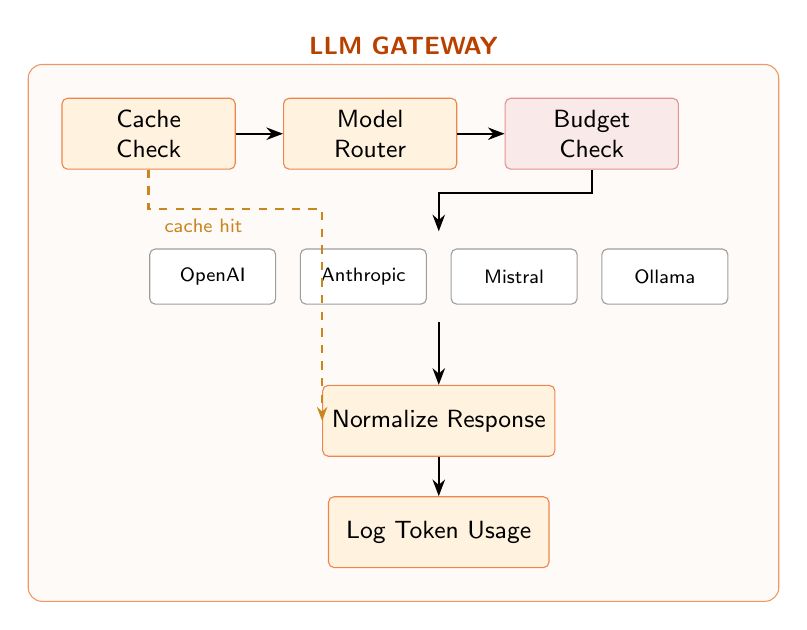
\begin{tikzpicture}[node distance=0.5cm and 0.5cm]

    % Gateway box
    \node[process, minimum width=2.2cm] (cache) {Cache\\Check};
    \node[process, minimum width=2.2cm, right=0.6cm of cache] (router) {Model\\Router};
    \node[process, minimum width=2.2cm, right=0.6cm of router, fill=costred!10, draw=costred!50] (budget) {Budget\\Check};

    % Providers
    \node[provider, below=1cm of router, xshift=-2cm] (openai) {OpenAI};
    \node[provider, right=0.3cm of openai] (anthropic) {Anthropic};
    \node[provider, right=0.3cm of anthropic] (mistral) {Mistral};
    \node[provider, right=0.3cm of mistral] (ollama) {Ollama};

    % Provider interface box
    \begin{scope}[on background layer]
        \node[rectangle, draw=compborder, fill=compbg, rounded corners=3pt,
              fit=(openai)(anthropic)(mistral)(ollama),
              inner sep=6pt,
              label={[font=\scriptsize\sffamily\bfseries]above:Provider Interface}] (provbox) {};
    \end{scope}

    % Normalize + Log
    \node[process, minimum width=2.8cm, below=0.8cm of provbox] (normalize) {Normalize Response};
    \node[process, minimum width=2.8cm, below=0.5cm of normalize] (logtoken) {Log Token Usage};

    % Flows
    \draw[data flow] (cache) -- (router);
    \draw[data flow] (router) -- (budget);
    \draw[data flow] (budget.south) -- ++(0,-0.3) -| (provbox.north);

    % Cache hit shortcut
    \draw[-{Stealth[length=5pt]}, thick, dashed, color=cachegold!80!black]
        (cache.south) -- ++(0,-0.5) -| node[below left, pos=0.3, font=\scriptsize\sffamily, text=cachegold!80!black] {cache hit} (normalize.west);

    \draw[data flow] (provbox) -- (normalize);
    \draw[data flow] (normalize) -- (logtoken);

    % Gateway bounding box
    \begin{scope}[on background layer]
        \node[rectangle, draw=accentorange!60, fill=accentorange!3,
              rounded corners=5pt, fit=(cache)(router)(budget)(provbox)(normalize)(logtoken),
              inner sep=12pt,
              label={[font=\small\sffamily\bfseries, text=accentorange!80!black]above:LLM GATEWAY}] {};
    \end{scope}

\end{tikzpicture}
\caption{LLM Gateway: request flow through cache, routing, budget check, and provider abstraction.}
\label{fig:llm-gateway}
\end{figure}

\textbf{Provider Interface} (abstract protocol):

\begin{lstlisting}[style=python, caption={Abstract LLM provider interface and normalized response type.}, label={lst:provider}]
class LLMProvider(Protocol):
    async def complete(
        self,
        messages: list[Message],
        model: str,
        temperature: float,
        max_tokens: int,
        response_format: ResponseFormat,
    ) -> LLMResponse: ...

@dataclass
class LLMResponse:
    content: str
    model: str
    provider: str
    usage: TokenUsage       # prompt_tokens, completion_tokens, total_tokens
    latency_ms: float
    cached: bool
    cost_usd: float         # Computed from token count * price
    request_id: str         # Provider-side request ID
    timestamp: datetime
\end{lstlisting}

Each provider implements this interface. The gateway normalizes all responses into the same format, regardless of the underlying API.

% ── 3.5 Prompt Engine ──
\subsection{Prompt Engine}

The framework uses \textbf{Jinja2} templates for prompt rendering, enabling conditionals, loops, and filters---significantly more powerful than simple string substitution.

\begin{lstlisting}[style=jinja, caption={System prompt template (simplified).}, label={lst:systemprompt}]
{# templates/system.j2 #}
You are {{ agent.persona.label }}.

## Your Background
{{ agent.persona.background }}

## Your Goals
- Primary: {{ agent.persona.goals.primary }}
{% if agent.persona.goals.secondary %}
- Secondary: {{ agent.persona.goals.secondary }}
{% endif %}

## Negotiation Context
{{ scenario.shared_context }}

## Participants
{% for other in visible_agents %}
- {{ other.label }} ({{ other.role }}): {{ other.public_description }}
{% endfor %}

## Your Constraints
{% for c in agent.persona.constraints %}
- {{ c }}
{% endfor %}

## Response Format
Respond exclusively in the following JSON format:
{{ response_schema_example }}
\end{lstlisting}

\textbf{Prompt compression} for advanced rounds reduces input tokens:
\begin{itemize}
    \item Rounds 1--3: Full history in prompt.
    \item Rounds 4+: Algorithmically compressed (last 2 rounds full + summary of earlier rounds) or summarized by a cheap model.
\end{itemize}

% ── 3.6 State Manager ──
\subsection{State Manager}

State is \textbf{immutable per round}---each round produces a new state snapshot. This enables full traceability, straightforward debugging (inspect any round's state), and safe parallelization without mutexes.

\begin{lstlisting}[style=python, caption={Immutable state data structures.}, label={lst:state}]
@dataclass(frozen=True)
class RoundState:
    round_number: int
    agents: tuple[AgentState, ...]
    decisions: tuple[Decision, ...]
    metrics: RoundMetrics
    timestamp: datetime

@dataclass(frozen=True)
class SimulationState:
    scenario_id: str
    repetition: int
    seed: int
    rounds: tuple[RoundState, ...]      # Append-only history
    cost_accumulated: CostSummary
    status: SimulationStatus            # running | completed | aborted | error
\end{lstlisting}

% ══════════════════════════════════════════════════════════
\section{Output Layer: Result Schemas}
\label{sec:output}
% ══════════════════════════════════════════════════════════

\subsection{Output Directory Structure}

\begin{lstlisting}[style=directory, caption={Output directory layout for a single run.}]
output/runs/peatland-exp-001_20260525_143022/
  manifest.json                     # Reproducibility manifest
  run_summary.json                  # Aggregated results
  config_snapshot/                  # Exact copy of all input files
    scenario.yaml
    personas/
      farmers.yaml
      authorities.yaml
      ngos.yaml
    run_config.yaml
  repetitions/
    rep_001/
      decisions.jsonl               # One line per agent decision
      rounds.json                   # Round summaries
      cost_log.jsonl                # Token/cost per API call
      agent_histories/
        farmer_conventional_large.json
        farmer_ecological_pioneer.json
        ...
      raw_responses/                # Unfiltered LLM outputs
        round_01/
          farmer_conventional_large.json
          ...
    rep_002/
      ...
  analysis/
    acceptance_by_persona.csv
    cost_breakdown.csv
    convergence.csv
  logs/
    framework.log
    errors.log
\end{lstlisting}

\subsection{Decision Log Schema (\texttt{decisions.jsonl})}

Each line is a self-contained JSON object representing one agent's decision in one round.

\begin{lstlisting}[style=json, caption={Decision log entry (one line in JSONL).}, label={lst:decision}]
{
  "decision_id": "d_001_r01_farmer_conv",
  "run_id": "peatland-exp-001",
  "repetition": 1,
  "round": 1,
  "agent_id": "farmer_conventional_large",
  "role": "farmer",
  "persona_id": "conventional_large",
  "timestamp": "2026-05-25T14:30:45.123Z",
  "decision": {
    "accept_rewetting": false,
    "conditions": {
      "min_compensation": 1400,
      "max_contract_years": 10,
      "requires_exit_clause": true
    },
    "message_to_others": "The offered compensation does not cover
      my crop losses. I need at least 1400 EUR per hectare per year."
  },
  "reasoning": "As a large farm with 60ha peatland, crop loss from
    rewetting would be substantial. The offered 800 EUR/ha is well
    below my break-even of approx. 1200 EUR/ha.",
  "prompt_tokens": 2134,
  "completion_tokens": 287,
  "model": "gpt-4o",
  "cost_usd": 0.0167,
  "latency_ms": 1423,
  "cached": false,
  "parse_retries": 0
}
\end{lstlisting}

\subsection{Cost Log Schema (\texttt{cost\_log.jsonl})}

\begin{lstlisting}[style=json, caption={Cost log entry per API call.}, label={lst:costlog}]
{
  "call_id": "c_001_r01_farmer_conv_decision",
  "timestamp": "2026-05-25T14:30:45.123Z",
  "repetition": 1,
  "round": 1,
  "agent_id": "farmer_conventional_large",
  "task": "decision",
  "provider": "openai",
  "model": "gpt-4o",
  "prompt_tokens": 2134,
  "completion_tokens": 287,
  "total_tokens": 2421,
  "cost_usd": 0.0167,
  "latency_ms": 1423,
  "cached": false,
  "cache_key_hash": "sha256:a1b2c3...",
  "retry_count": 0,
  "error": null
}
\end{lstlisting}

\subsection{Reproducibility Manifest (\texttt{manifest.json})}

Contains everything needed to reproduce the run exactly.

\begin{lstlisting}[style=json, caption={Reproducibility manifest (abbreviated).}, label={lst:manifest}]
{
  "manifest_version": "1.0",
  "run_id": "peatland-exp-001",
  "timestamp_start": "2026-05-25T14:30:22Z",
  "timestamp_end": "2026-05-25T14:47:13Z",
  "duration_seconds": 1011,
  "reproducibility": {
    "seed": 42,
    "config_hash": "sha256:e4f5a6b7...",
    "scenario_hash": "sha256:1a2b3c4d...",
    "personas_hash": "sha256:5e6f7a8b...",
    "framework_version": "0.1.0",
    "framework_git_commit": "abc1234",
    "python_version": "3.12.4",
    "dependency_lock_hash": "sha256:9c0d1e2f..."
  },
  "environment": {
    "os": "macOS 15.2",
    "cpu": "Apple M3 Pro",
    "ram_gb": 18
  },
  "llm_models_used": [
    {
      "provider": "openai",
      "model": "gpt-4o",
      "model_version": "gpt-4o-2024-08-06",
      "tasks": ["decision"],
      "total_calls": 120,
      "total_tokens": 287400,
      "total_cost_usd": 2.14
    }
  ],
  "totals": {
    "repetitions_completed": 10,
    "total_rounds": 73,
    "total_api_calls": 160,
    "total_tokens": 339400,
    "total_cost_usd": 2.22,
    "cache_hit_rate": 0.12
  }
}
\end{lstlisting}

\subsection{Run Summary (\texttt{run\_summary.json})}

Aggregated results across all repetitions.

\begin{lstlisting}[style=json, caption={Run summary with per-persona results.}, label={lst:runsummary}]
{
  "run_id": "peatland-exp-001",
  "per_persona_results": [
    {
      "persona_id": "conventional_large",
      "acceptance_rate": 0.30,
      "avg_min_compensation_demanded": 1380,
      "most_effective_incentive": "regulatory_pressure",
      "decision_variance": 0.15
    },
    {
      "persona_id": "ecological_pioneer",
      "acceptance_rate": 1.00,
      "avg_min_compensation_demanded": 420,
      "most_effective_incentive": "compensation",
      "decision_variance": 0.03
    },
    {
      "persona_id": "skeptical_traditional",
      "acceptance_rate": 0.20,
      "avg_min_compensation_demanded": 1850,
      "most_effective_incentive": "regulatory_pressure",
      "decision_variance": 0.22
    }
  ],
  "aggregate": {
    "overall_acceptance_rate": 0.575,
    "cost_per_simulation_usd": 0.222,
    "tokens_per_decision": 2421,
    "avg_rounds_to_termination": 6.2
  }
}
\end{lstlisting}

% ══════════════════════════════════════════════════════════
\section{Technology Stack}
\label{sec:techstack}
% ══════════════════════════════════════════════════════════

\begin{table}[H]
\centering
\begin{tabularx}{\textwidth}{llX}
    \toprule
    \textbf{Component} & \textbf{Technology} & \textbf{Rationale} \\
    \midrule
    Language            & Python 3.12+            & Ecosystem, LLM libraries, scientific stack \\
    Data models         & Pydantic v2             & Validation, serialization, JSON Schema generation \\
    Prompt templates    & Jinja2                  & Conditionals, loops, filters \\
    LLM clients         & Official SDKs           & \texttt{openai}, \texttt{anthropic}, \texttt{mistralai} \\
    Async I/O           & \texttt{asyncio}/\texttt{httpx} & Parallel API calls without thread overhead \\
    Config              & PyYAML + jsonschema     & YAML parsing + strict schema validation \\
    Caching             & SQLite (\texttt{aiosqlite}) & Lightweight, no external service \\
    CLI                 & \texttt{typer}          & Modern CLI with auto-documentation \\
    Logging             & \texttt{structlog}      & JSON logging for machine-readable output \\
    Testing             & \texttt{pytest}         & \texttt{pytest-asyncio} for async tests \\
    Analysis            & pandas + matplotlib     & Basic analysis and visualization \\
    \bottomrule
\end{tabularx}
\caption{Core technology stack.}
\label{tab:techstack}
\end{table}

\begin{table}[H]
\centering
\begin{tabularx}{\textwidth}{llX}
    \toprule
    \textbf{Component} & \textbf{Technology} & \textbf{When Needed} \\
    \midrule
    Experiment tracking & MLflow / W\&B       & Comparing across many runs \\
    Dashboard           & Streamlit           & Interactive result exploration \\
    Distributed cache   & Redis               & High parallelism, multi-machine setups \\
    \bottomrule
\end{tabularx}
\caption{Optional extensions (not part of core).}
\label{tab:techstack-opt}
\end{table}

% ══════════════════════════════════════════════════════════
\section{End-to-End Data Flow}
\label{sec:dataflow}
% ══════════════════════════════════════════════════════════

\begin{figure}[H]
\centering
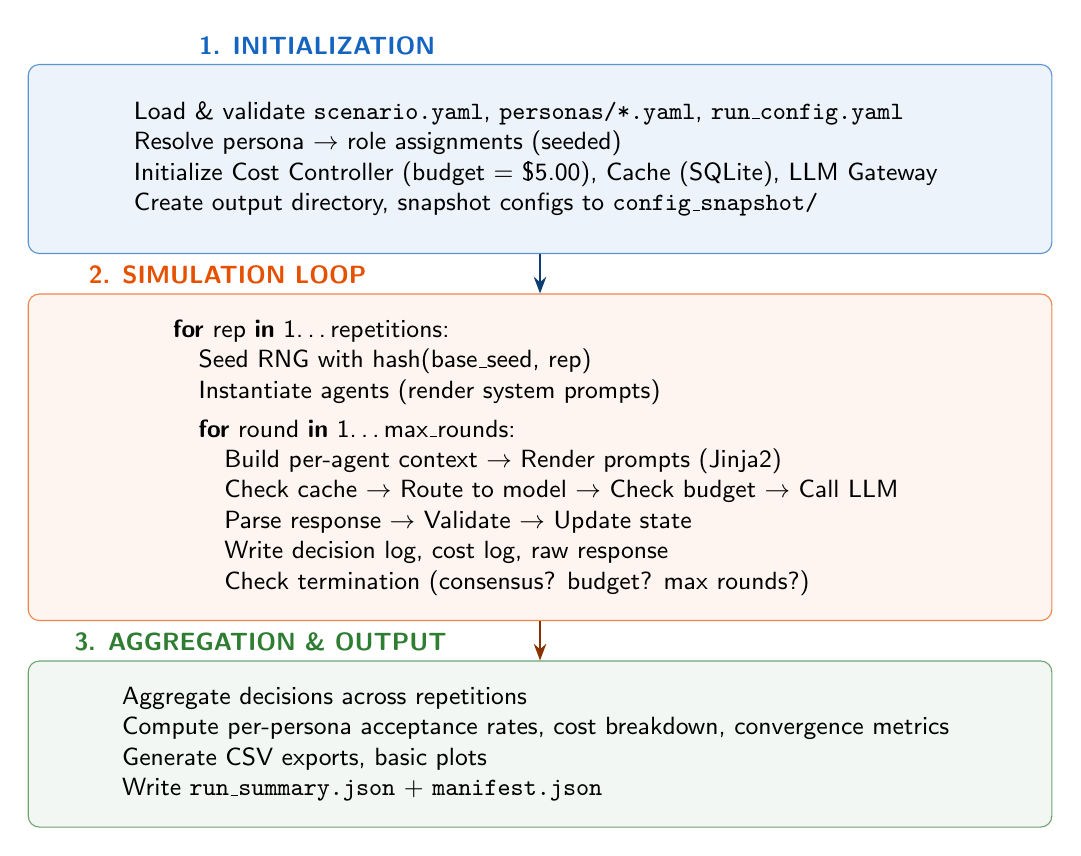
\begin{tikzpicture}[node distance=0.4cm, every node/.style={font=\small\sffamily}]

    % Phase 1: Init
    \node[rectangle, draw=accentblue!70, fill=accentblue!8, rounded corners=4pt,
          minimum width=13cm, minimum height=2.4cm, align=left, inner sep=8pt,
          label={[font=\small\sffamily\bfseries, text=accentblue]above left:1. INITIALIZATION}] (init) {
        \begin{tabular}{@{}l@{}}
            Load \& validate \texttt{scenario.yaml}, \texttt{personas/*.yaml}, \texttt{run\_config.yaml} \\
            Resolve persona $\to$ role assignments (seeded) \\
            Initialize Cost Controller (budget = \$5.00), Cache (SQLite), LLM Gateway \\
            Create output directory, snapshot configs to \texttt{config\_snapshot/}
        \end{tabular}
    };

    % Phase 2: Simulation
    \node[rectangle, draw=accentorange!70, fill=accentorange!6, rounded corners=4pt,
          minimum width=13cm, minimum height=3.6cm, align=left, inner sep=8pt,
          below=0.5cm of init,
          label={[font=\small\sffamily\bfseries, text=accentorange]above left:2. SIMULATION LOOP}] (sim) {
        \begin{tabular}{@{}l@{}}
            \textbf{for} rep \textbf{in} 1\ldots repetitions: \\
            \quad Seed RNG with hash(base\_seed, rep) \\
            \quad Instantiate agents (render system prompts) \\[3pt]
            \quad \textbf{for} round \textbf{in} 1\ldots max\_rounds: \\
            \quad\quad Build per-agent context $\to$ Render prompts (Jinja2) \\
            \quad\quad Check cache $\to$ Route to model $\to$ Check budget $\to$ Call LLM \\
            \quad\quad Parse response $\to$ Validate $\to$ Update state \\
            \quad\quad Write decision log, cost log, raw response \\
            \quad\quad Check termination (consensus? budget? max rounds?)
        \end{tabular}
    };

    % Phase 3: Aggregation
    \node[rectangle, draw=accentgreen!70, fill=accentgreen!6, rounded corners=4pt,
          minimum width=13cm, minimum height=2cm, align=left, inner sep=8pt,
          below=0.5cm of sim,
          label={[font=\small\sffamily\bfseries, text=accentgreen]above left:3. AGGREGATION \& OUTPUT}] (agg) {
        \begin{tabular}{@{}l@{}}
            Aggregate decisions across repetitions \\
            Compute per-persona acceptance rates, cost breakdown, convergence metrics \\
            Generate CSV exports, basic plots \\
            Write \texttt{run\_summary.json} + \texttt{manifest.json}
        \end{tabular}
    };

    \draw[data flow=accentblue] (init) -- (sim);
    \draw[data flow=accentorange] (sim) -- (agg);

\end{tikzpicture}
\caption{End-to-end data flow from initialization through simulation to output.}
\label{fig:dataflow}
\end{figure}

\textbf{CLI invocation:}
\begin{lstlisting}[style=directory]
$ framework run --scenario scenario.yaml --config run_config.yaml
\end{lstlisting}

% ══════════════════════════════════════════════════════════
\section{Cost Optimization Mechanisms}
\label{sec:cost}
% ══════════════════════════════════════════════════════════

Cost optimization is a central contribution of this thesis. The following strategies are applied in layers, each building on the previous.

\subsection{Cost Reduction Waterfall}

\begin{figure}[H]
\centering
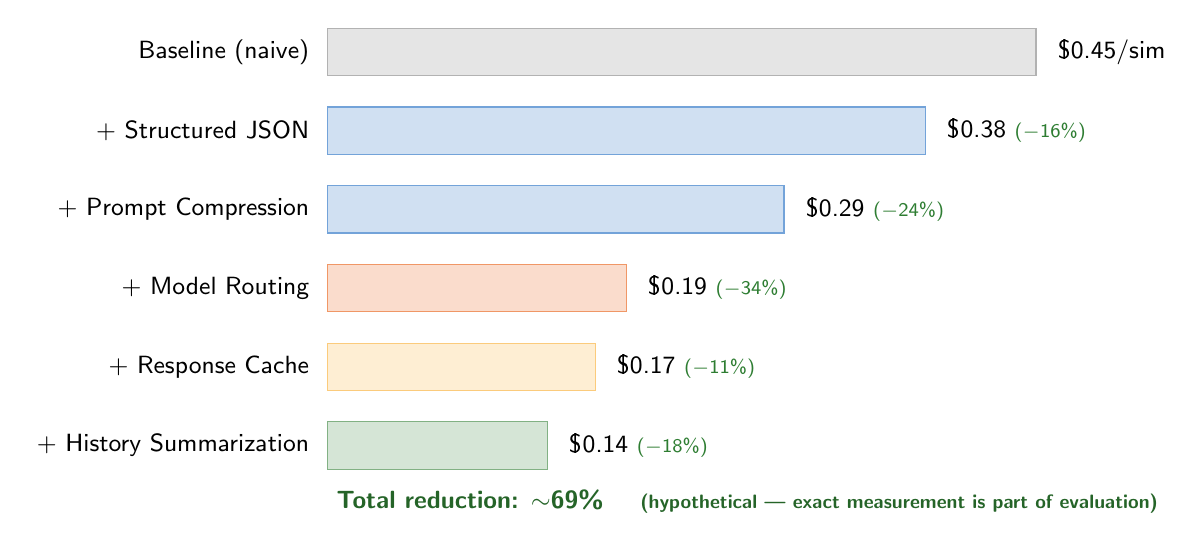
\begin{tikzpicture}[
    bar/.style={rectangle, draw=#1!60, fill=#1!20, minimum height=0.6cm, anchor=west, font=\small\sffamily},
]
    % Baseline
    \node[bar=gray, minimum width=9cm] (b0) at (0, 5) {};
    \node[left=0.1cm of b0, font=\small\sffamily, anchor=east] {Baseline (naive)};
    \node[right=0.15cm of b0, font=\small\sffamily] {\$0.45/sim};

    % + Structured JSON
    \node[bar=accentblue, minimum width=7.6cm] (b1) at (0, 4) {};
    \node[left=0.1cm of b1, font=\small\sffamily, anchor=east] {+ Structured JSON};
    \node[right=0.15cm of b1, font=\small\sffamily] {\$0.38 \textcolor{accentgreen}{\scriptsize($-$16\%)}};

    % + Prompt Compression
    \node[bar=accentblue, minimum width=5.8cm] (b2) at (0, 3) {};
    \node[left=0.1cm of b2, font=\small\sffamily, anchor=east] {+ Prompt Compression};
    \node[right=0.15cm of b2, font=\small\sffamily] {\$0.29 \textcolor{accentgreen}{\scriptsize($-$24\%)}};

    % + Model Routing
    \node[bar=accentorange, minimum width=3.8cm] (b3) at (0, 2) {};
    \node[left=0.1cm of b3, font=\small\sffamily, anchor=east] {+ Model Routing};
    \node[right=0.15cm of b3, font=\small\sffamily] {\$0.19 \textcolor{accentgreen}{\scriptsize($-$34\%)}};

    % + Response Cache
    \node[bar=cachegold, minimum width=3.4cm] (b4) at (0, 1) {};
    \node[left=0.1cm of b4, font=\small\sffamily, anchor=east] {+ Response Cache};
    \node[right=0.15cm of b4, font=\small\sffamily] {\$0.17 \textcolor{accentgreen}{\scriptsize($-$11\%)}};

    % + History Summarization
    \node[bar=accentgreen, minimum width=2.8cm] (b5) at (0, 0) {};
    \node[left=0.1cm of b5, font=\small\sffamily, anchor=east] {+ History Summarization};
    \node[right=0.15cm of b5, font=\small\sffamily] {\$0.14 \textcolor{accentgreen}{\scriptsize($-$18\%)}};

    % Total label
    \node[below=0.4cm of b5.south west, font=\small\sffamily\bfseries, anchor=west, text=accentgreen!80!black] {
        Total reduction: $\sim$69\% \quad\textit{\scriptsize(hypothetical --- exact measurement is part of evaluation)}
    };

\end{tikzpicture}
\caption{Cumulative cost reduction waterfall across optimization strategies.}
\label{fig:cost-waterfall}
\end{figure}

\subsection{Optimization Strategies Detail}

\begin{table}[H]
\centering
\small
\begin{tabularx}{\textwidth}{clXl}
    \toprule
    \textbf{\#} & \textbf{Strategy} & \textbf{Mechanism} & \textbf{Expected Impact} \\
    \midrule
    1 & Structured Output &
        \texttt{response\_format: json} or tool-use instead of free-text parsing &
        Eliminates 5--15\% retries \\
    2 & Prompt Compression &
        Summarize history in late rounds instead of full embedding &
        $-$30--60\% input tokens (round 4+) \\
    3 & Model Routing &
        Strong model for decisions; cheap model for summaries &
        $-$40--70\% cost for sub-tasks \\
    4 & Response Cache &
        SHA-256 over (system + user prompt) $\to$ cache lookup &
        Effective when \texttt{repetitions > 1} \\
    5 & Token Budget &
        Hard limit per response, per round, per run &
        Prevents runaway costs \\
    6 & Batch API &
        OpenAI Batch API (50\% discount, 24h SLA) &
        $-$50\% for non-time-critical runs \\
    7 & Local Models &
        Ollama fallback for dev/testing &
        \$0 during development \\
    \bottomrule
\end{tabularx}
\caption{Cost optimization strategies and expected impact.}
\label{tab:cost-strategies}
\end{table}

\subsection{Cost Controller Architecture}

\begin{figure}[H]
\centering
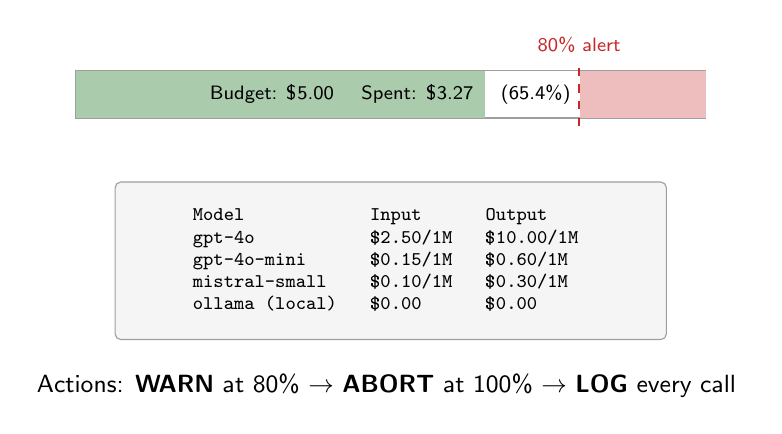
\begin{tikzpicture}[node distance=0.3cm]

    % Budget bar
    \node[rectangle, draw=compborder, fill=white, minimum width=8cm, minimum height=0.6cm, anchor=west] (budgetbg) at (0, 0) {};
    \node[rectangle, fill=accentgreen!40, minimum width=5.2cm, minimum height=0.6cm, anchor=west] (budgetfill) at (0, 0) {};
    \node[rectangle, fill=costred!30, minimum width=1.6cm, minimum height=0.6cm, anchor=west] at (6.4cm, 0) {};
    \node[font=\scriptsize\sffamily] at (4cm, 0) {Budget: \$5.00 \quad Spent: \$3.27 \quad (65.4\%)};

    % Warning line
    \draw[dashed, thick, costred] (6.4cm, -0.4) -- (6.4cm, 0.4) node[above, font=\scriptsize\sffamily, text=costred] {80\% alert};

    % Price table
    \node[rectangle, draw=compborder, fill=compbg, rounded corners=2pt,
          minimum width=7cm, minimum height=2cm, align=left, inner sep=6pt,
          below=0.8cm of budgetbg, font=\scriptsize\ttfamily] (prices) {
        \begin{tabular}{lll}
            \textbf{Model} & \textbf{Input} & \textbf{Output} \\
            gpt-4o & \$2.50/1M & \$10.00/1M \\
            gpt-4o-mini & \$0.15/1M & \$0.60/1M \\
            mistral-small & \$0.10/1M & \$0.30/1M \\
            ollama (local) & \$0.00 & \$0.00 \\
        \end{tabular}
    };

    % Actions
    \node[below=0.3cm of prices, font=\small\sffamily, align=left] (actions) {
        Actions: \textbf{WARN} at 80\% $\to$ \textbf{ABORT} at 100\% $\to$ \textbf{LOG} every call
    };

\end{tikzpicture}
\caption{Cost Controller: budget tracking with configurable price table and alert thresholds.}
\label{fig:cost-controller}
\end{figure}

% ══════════════════════════════════════════════════════════
\section{Reproducibility and Hashing}
\label{sec:reproducibility}
% ══════════════════════════════════════════════════════════

\subsection{Configuration Hashing}

Each run receives a deterministic hash over all inputs:

$$
\texttt{config\_hash} = \text{SHA-256}\!\Big(\text{canonical\_json}(\texttt{scenario}) \;\|\; \text{canonical\_json}(\texttt{personas}) \;\|\; \text{canonical\_json}(\texttt{run\_config})\Big)
$$

\textbf{Canonical JSON}: YAML is converted to sorted, indentation-normalized JSON before hashing. This ensures that cosmetic YAML changes (comments, indentation) do not alter the hash.

\subsection{Seed Strategy}

\begin{figure}[H]
\centering
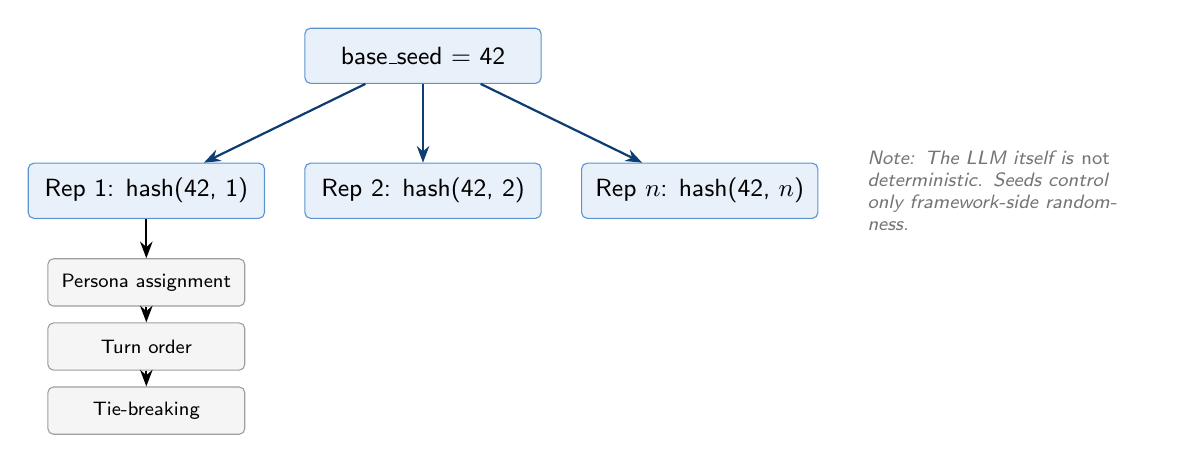
\begin{tikzpicture}[
    seed/.style={rectangle, draw=accentblue!70, fill=accentblue!10, rounded corners=2pt, minimum height=0.7cm,
                 minimum width=3cm, font=\small\sffamily, align=center},
    derived/.style={rectangle, draw=compborder, fill=compbg, rounded corners=2pt, minimum height=0.6cm,
                    minimum width=2.5cm, font=\scriptsize\sffamily, align=center},
]
    \node[seed] (base) {base\_seed = 42};

    \node[seed, below left=1cm and 0.5cm of base] (r1) {Rep 1: hash(42, 1)};
    \node[seed, below=1cm of base] (r2) {Rep 2: hash(42, 2)};
    \node[seed, below right=1cm and 0.5cm of base] (rn) {Rep $n$: hash(42, $n$)};

    \node[derived, below=0.5cm of r1] (r1a) {Persona assignment};
    \node[derived, below=0.2cm of r1a] (r1b) {Turn order};
    \node[derived, below=0.2cm of r1b] (r1c) {Tie-breaking};

    \draw[data flow=accentblue] (base) -- (r1);
    \draw[data flow=accentblue] (base) -- (r2);
    \draw[data flow=accentblue] (base) -- (rn);
    \draw[data flow] (r1) -- (r1a);
    \draw[data flow] (r1a) -- (r1b);
    \draw[data flow] (r1b) -- (r1c);

    \node[right=0.5cm of rn, font=\scriptsize\sffamily\itshape, text=yamlcomment, text width=3.5cm] {
        Note: The LLM itself is \emph{not} deterministic. Seeds control only framework-side randomness.
    };
\end{tikzpicture}
\caption{Seed derivation strategy: base seed is combined with repetition index.}
\label{fig:seed}
\end{figure}

\subsection{Reproducibility Artifacts}

\begin{table}[H]
\centering
\begin{tabularx}{\textwidth}{lX}
    \toprule
    \textbf{Artifact} & \textbf{Purpose} \\
    \midrule
    \texttt{config\_snapshot/} & Exact copy of all input files \\
    \texttt{manifest.json $\to$ config\_hash} & Identify identical configurations \\
    \texttt{manifest.json $\to$ framework\_git\_commit} & Framework version \\
    \texttt{manifest.json $\to$ dependency\_lock\_hash} & Exact dependency versions \\
    \texttt{manifest.json $\to$ llm\_models\_used[].model\_version} & Exact model version \\
    \texttt{raw\_responses/} & Unfiltered API responses \\
    \texttt{cost\_log.jsonl $\to$ cache\_key\_hash} & Traceable which calls were cached \\
    \bottomrule
\end{tabularx}
\caption{Artifacts logged for reproducibility.}
\label{tab:reproducibility}
\end{table}

\textbf{Key insight}: Since LLMs are non-deterministic even at temperature~0, \texttt{repetitions > 1} is required for statistical validity. The seed controls only framework-side random decisions (persona assignment, turn ordering, tie-breaking).

% ══════════════════════════════════════════════════════════
\section{Open Design Decisions}
\label{sec:open}
% ══════════════════════════════════════════════════════════

The following decisions remain open and will be resolved during implementation:

\begin{enumerate}
    \item \textbf{Template language}: Jinja2 is powerful but complex. Would a simpler mechanism (e.g., Python f-strings with sandboxing) suffice?
    \item \textbf{State persistence}: Should state be persisted during the run (for crash recovery), or only written at completion?
    \item \textbf{Streaming}: Should LLM responses be streamed (for live monitoring), or is batch collection sufficient?
    \item \textbf{Plugin system}: Should there be a plugin interface for custom topologies, providers, and metrics, or does inheritance suffice?
    \item \textbf{Scenario-level validation}: Should the framework validate domain-specific constraints (e.g., ``authority budget covers offered compensation''), or is that the scenario author's responsibility?
    \item \textbf{Prompt language}: Should prompts be in English or German? Language-dependence of results as an evaluation point?
\end{enumerate}

\end{document}
